% Intended LaTeX compiler: pdflatex
\documentclass[10pt,a4paper,UTF8]{article}
\usepackage{zclorg}
\author{张朝龙}
\date{}
\title{学习Python Doc第七天: 错误和例外}
\hypersetup{
 pdfauthor={张朝龙},
 pdftitle={学习Python Doc第七天: 错误和例外},
 pdfkeywords={},
 pdfsubject={},
 pdfcreator={Emacs 25.0.50.1 (Org mode 9.0.5)}, 
 pdflang={English}}
\begin{document}

\maketitle
\tableofcontents
\titlepic{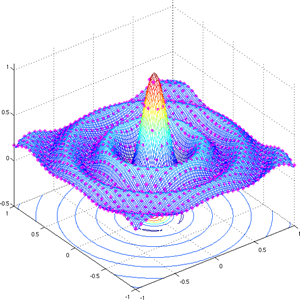
\includegraphics[scale=0.25]{../../img/sinc.PNG}}
截至目前,我们见过 \texttt{Python} 的报错信息,但是我们还没有涉及 \texttt{Python} 的错误和例外处理机制。在python中有两类错误: 语法错误和例外。

\section{语法错误}
\label{sec:org1e36fdb}


语法错误可能是最常见的错误,也做好调试。
\lstset{language=Python,label= ,caption= ,captionpos=b,numbers=none}
\begin{lstlisting}
while True print('hello world')
\end{lstlisting}

显示报错信息:
\begin{verbatim}
    while True print('hello world')
                   ^
SyntaxError: invalid syntax
\end{verbatim}
解释器会提示报错信息。
\section{例外}
\label{sec:org6fe6da7}


即便一个表达式语法正确,其执行过程中仍然可能导致错误。执行过程中的错误叫做例外。

先看几个例外。
\begin{enumerate}
\item 除零
\end{enumerate}
\begin{verbatim}
>>> 10*(1/0)
ZeroDivisionError: division by zero
\end{verbatim}
\begin{enumerate}
\item 变量未定义
\end{enumerate}

\begin{verbatim}
>>> 4 + spam*3
NameError: name 'spam' is not defined
\end{verbatim}

\begin{enumerate}
\item 类型不匹配
\end{enumerate}

\begin{verbatim}
>>> '2' + 2
TypeError: Can't convert 'int' object to str implicitly
\end{verbatim}
在以上的三个例子中,出现的例外有: \texttt{ZeroDivisionError} ,  \texttt{NameError} , \texttt{TypeError} . 这三个例外的名字是事先定义好的。Python有许多内置的例外信息可以点击\href{https://docs.python.org/3.5/library/exceptions.html\#bltin-exceptions}{这里} 查询。

\section{处理例外}
\label{sec:orgb3b9161}


编写程序时可以针对特定的例外执行相关操作。看代码:
\lstset{language=Python,label= ,caption= ,captionpos=b,numbers=none}
\begin{lstlisting}
while True:
    try:
        x = int(input("please enter a number:"))
    except ValueError:
        print("Oops! That was no valid number. Try again")
\end{lstlisting}

整个程序执行顺序是:
\begin{enumerate}
\item 在 \texttt{try} 和 \texttt{except} 之间的语句首先执行。
\item 如果没有例外发生, \texttt{except} 之后的语句就会被跳过。
\item 如果例外发生,并且类型和 \texttt{except} 之后的类型一样(本例中是 \texttt{ValueError} )。 \texttt{except} 后面的语句被执行。
\item 如果例外发生,但是类型和 \texttt{except} 后面的类型不同,那么这个例外就是未处理例外,程序停止执行。
\end{enumerate}

一个 \texttt{try} 可以有多个例外语句。一个 \texttt{except} 语句可以包含多个例外关键词。看代码:
\lstset{language=Python,label= ,caption= ,captionpos=b,numbers=none}
\begin{lstlisting}
import sys

try:
    f = open('myfile.txt')
    s = f.readline()
    i = int(s.strip())
except OSError as err:
    print("OS error: {0}".format(err))
except ValueError:
    print("Could not convert data to an integer.")
except:
    print("Unexpected error:", sys.exc_info()[0])
    raise
\end{lstlisting}

另外 \texttt{try except} 语句可以有 \texttt{else} ,看代码:
\lstset{language=Python,label= ,caption= ,captionpos=b,numbers=none}
\begin{lstlisting}
for arg in sys.argv[1:]:
    try:
        f = open(arg, 'r')
    except IOError:
        print('cannot open', arg)
    else:
        print(arg, 'has', len(f.readlines()), 'lines')
        f.close()
\end{lstlisting}

\section{发起一个例外}
\label{sec:org970a446}


\texttt{raise} 语句强制程序发起例外。看代码:

\lstset{language=Python,label= ,caption= ,captionpos=b,numbers=none}
\begin{lstlisting}
raise NameError('HiThere')
\end{lstlisting}

\section{用户定义例外}
\label{sec:orgc74ee1d}


通过创建一个新的例外类(一切都是对象,所有的例外类都应当从 \texttt{Exception} 继承而来。) 程序可以命名自己的例外。 

可以定义例外类,这个例外类可以做其他类能做的一切。通过创建一个基类,可以创建一个可以处理多个不同错误的模块。每个基于这个基类的子类负责处理特定的例外。看代码:

\lstset{language=Python,label= ,caption= ,captionpos=b,numbers=none}
\begin{lstlisting}
class Error(Exception):
    """Base class for exceptions in this module."""
    pass

class InputError(Error):
    """Exception raised for errors in the input.

    Attributes:
        expression -- input expression in which the error occurred
        message -- explanation of the error
    """

    def __init__(self, expression, message):
        self.expression = expression
        self.message = message

class TransitionError(Error):
    """Raised when an operation attempts a state transition that's not
    allowed.

    Attributes:
        previous -- state at beginning of transition
        next -- attempted new state
        message -- explanation of why the specific transition is not allowed
    """

    def __init__(self, previous, next, message):
        self.previous = previous
        self.next = next
        self.message = message
\end{lstlisting}

每个例外都是基于 \texttt{Error} 这个类来的。

\section{定义 \texttt{clean-up} 动作}
\label{sec:orgec5b440}


\texttt{try} 语句有另外一个可选的语句 \texttt{finally} ,专门用来定义清理动作。清理动作在所有情况之后执行。看代码:

\lstset{language=Python,label= ,caption= ,captionpos=b,numbers=none}
\begin{lstlisting}
try:
    raise KeyboardInterrupt
finally:
    print('Goodbye, world')
\end{lstlisting}

\texttt{finally} 语句在离开 \texttt{try} 语句之后必须不管是否有例外发生都执行。看代码:
\lstset{language=Python,label= ,caption= ,captionpos=b,firstnumber=1,numbers=left}
\begin{lstlisting}
def divide(x,y):
    try:
        result = x/y
    except ZeroDivisionError:
        print("division by zero")
    else:
        print("result is ",result)
    finally:
        print("executing finally clause")
\end{lstlisting}
输出是:

\begin{verbatim}
In [3]: divide(2,1)
result is  2.0
executing finally clause

In [11]: divide(2,0)
division by zero
executing finally clause
\end{verbatim}

我们可以看到无论如何 \texttt{finally} 的语句都会执行。

\section{预先定义 \texttt{clean-up} 动作}
\label{sec:org0721662}


有些类定义了标准的 \texttt{clean-up} 动作。下面的代码打开一个文件,打印其内容到屏幕:
\lstset{language=Python,label= ,caption= ,captionpos=b,numbers=none}
\begin{lstlisting}
for line in open ("myfile.txt"):
    print(line,end="")
\end{lstlisting}

这段代码的问题是:代码执行结束之后,文件会保持打开状态一段时间。对于简单的脚本而言不是什么问题,但是对于较大的应用,这个可能会导致问题。  \texttt{with} 语句允许像 \texttt{file} 这样的对象一直处于clean up状态。

\lstset{language=Python,label= ,caption= ,captionpos=b,firstnumber=1,numbers=left}
\begin{lstlisting}
with open("myfile.txt") as f:
    for line in f:
        print(line, end="")
\end{lstlisting}

代码执行之后,文件 \texttt{f} 总是关闭的(即使在处理文件过程中发生问题。)。
\end{document}
